

\newpage
\chapter{Ohmsches Gesetz}


Bis jetzt haben wir uns mit der Stromstärke- und Spannungsmessung beschäftigt.
Man kann sich nun die Frage stellen, ob die Spannung und die Stromstärke
unabhängig voneinander sind oder nicht.

Denkt man an das Modell des Wasserkreislaufs, siehe \fref{fig:watermodel},
so wird klar, dass die Höhe des Wassers im Tank einen Einfluss auf die
Flussgeschwindigkeit des Wassers in den Röhren hat.
Es könnte also plausibel sein, dass die Spannung und die Stromstärke nicht
unabhängig voneinander sind.

\section{Der Schiebewiderstand}

Ein Schiebewiderstand ist ein elektrisches Bauteil, mit welchem man die Stromstärke
regulieren kann, siehe \fref{fig:potentiometer}. Er besteht aus einer gewickelten Spule
aus einem speziellen Widerstandsdraht und einem Schieber, der mit dieser Spule Kontakt hat.

\begin{figure}[h!]
    \centering
    \includegraphics[width=11cm]{_images/schiebewiderstand.pdf}
    \caption{Schiebewiderstand}
    \label{fig:potentiometer}
\end{figure}

Die Anschlüsse A und B sind miteinander und mit dem Schieber verbunden.
Die Anschlüsse der Spule sind bei C und D. Der Kontaktpunkt zwischen Schieber und Spule ist bei M.



\newpage
\experiment{Stromregulierung mit dem Schiebewiderstand}

Baue das Experiment aus siehe \fref{fig:potentiometer_series} auf.

\begin{figure}[h!]
    \centering
    \includegraphics[width=9cm]{_images/ohm_schiebewiderstand.pdf}
    \caption{Regulierung der Stromstärke mit dem Schiebewiderstand}
    \label{fig:potentiometer_series}
\end{figure}

Schliesse den Schalter und notiere deine Beobachtungen. Beantworte die folgenden Fragen:

\begin{enumerate}
    \item Miss die Stromstärke, wenn der Schieber ganz links ist.
    \item Miss die Stromstärke, wenn der Schieber in der Mitte ist.
    \item Miss die Stromstärke, wenn der Schieber ganz rechts ist.
    \item Vervollständige den Schaltplan.
\end{enumerate}


% Raster für die Antworten
\begin{tikzpicture}
    \draw[step=4mm,gray,very thin] (0,0) grid (14.8,-8.4);

    \noanswer{
        \node  at (7,-6)
            {\includegraphics[width=6cm]{_images/ohm_schiebewiderstand_schaltplan.pdf}};
    }

    \answer{
        \node  at (7,-6)
            {\includegraphics[width=6cm]{_images/ohm_schiebewiderstand_schaltplan_loesung.pdf}};
    }

    \answer{
        \draw (0.3,0.14) node[anchor=north west,align=left,text width=13cm] {%
      		\marker%

            \textbf{1.} Es fliessen ca. 0.26 A. \\
            \textbf{2.} Der Ausschlag der Nadel ist beim 3 A-Bereich kleiner Es fliesen etwas mehr als 0.2 A.\\
            \textbf{3.} Die Nadel schlägt in die negative Richtung aus.\\

        };
    }
\end{tikzpicture}






\newpage
\experiment{Zusammenhang zwischen Spannung und Stromstärke}

Baue das Experiment aus siehe \fref{fig:ohm_law} auf. Es gibt vier verschiedene
Widerstände auf dem Brettchen. Verbinde zuerst den zweitobersten
Widerstand ($\qty{10}{\ohm}$), danach den untersten ($\qty{20}{\ohm}$).

\begin{figure}[h!]
    \centering
    \includegraphics[width=9cm]{_images/ohm_gesetz.pdf}
    \caption{Strom- und Spannungsmessung über einem Widerstand.}
    \label{fig:ohm_law}
\end{figure}

Schliesse den Schalter und verändere den Schiebewiderstand. Miss vier verschiedene
Kombinationen von Spannung und Stromstärke. Zeichne anschliessend die Messwerte
in das Diagramm.

% Raster für die Antworten
\begin{tikzpicture}
    \draw[step=4mm,gray,very thin] (0,0) grid (14.8,-11.6);


    \begin{scope}[shift={(1.2,0)}]
    \draw (2.2,-0.6) node[anchor=north east,align=right,text width=3cm] {%
  		\markertable%
        U in V
        \ \\
        10 Ω , I in A
        \ \\
        20 Ω , I in A
        \ \\
    };

    \draw[very thick] (0.8,-1.6) -- (10.8,-1.6);

    \draw[very thick] (2.8,-0.4) -- ++(0,-3.6);

    \draw (3.6,-0.6) node[anchor=north,align=center,text width=2cm] {%
  		\markertable%
        0
        \ \\
        \answer{0}
        \ \\
        \answer{0}
        \ \\
    };


    \draw[very thick] (4.4,-0.4) -- ++(0,-3.6);

    \draw (5.2,-0.6) node[anchor=north,align=center,text width=2cm] {%
  		\markertable%
        0.5
        \ \\
        \answer{0.05}
        \ \\
        \answer{0}
        \ \\
    };

    \draw[very thick] (6,-0.4) -- ++(0,-3.6);

    \draw (6.8,-0.6) node[anchor=north,align=center,text width=2cm] {%
  		\markertable%
        1
        \ \\
        \answer{0.1}
        \ \\
        \answer{0}
        \ \\
    };

    \draw[very thick] (7.6,-0.4) -- ++(0,-3.6);

    \draw (8.4,-0.6) node[anchor=north,align=center,text width=2cm] {%
  		\markertable%
        1.5
        \ \\
        \answer{0.15}
        \ \\
        \answer{0}
        \ \\
    };

    \draw[very thick] (9.2,-0.4) -- ++(0,-3.6);

    \draw (10,-0.6) node[anchor=north,align=center,text width=2cm] {%
  		\markertable%
        \answer{2.2}
        \ \\
        \answer{0.22}
        \ \\
        \answer{0}
        \ \\
    };
    \end{scope}



    \begin{scope}[shift={(4,-10)}]
        \draw[color=white,fill=white] (-1,-1) rectangle (7,5);
        \begin{axis}[
                axis background/.style={fill=white},
                axis lines=left,
                xlabel=$I$ in A,
                ylabel=$U$ in V,
                xtick={0,0.1,0.2,0.3,0.4},
                ytick={0,1,2,3},
                minor tick num=1,
                grid=both,
                xmin=0.0, xmax=0.3,
                ymin=0, ymax=3,
                line width=1pt,
                height=6cm,
                width=8cm,
                domain=0:0.3,
                legend pos=south east
            ]
            \answer{
                \addplot[
                    mark=*, mark size=1.5,color=blue,
                ] coordinates
                {
                    (0,0)
                    (0.05, 0.5)
                    (0.1,1)
                    (0.15,1.5)
                    (0.22,2.2)
                };
                \addplot[
                    mark=*, mark size=1.5,color=red,
                ] coordinates
                {
                    (0,0)
                    (0.033, 0.5)
                    (0.067,1)
                    (0.1,1.5)
                    (0.15,2.2)
                };
                \legend{10 Ω,20 Ω}
            }
        \end{axis}
    \end{scope}

\end{tikzpicture}






\newpage
\section{Der elektrische Widerstand}

Der elektrische Widerstand $R$ ist definiert als das Verhältnis zwischen
der Spannung $U$ und der Stromstärke $I$. Die Einheit des Widerstands ist
das Ohm ($\unit{\ohm}$).

\begin{greenbox}
\textbf{Elektrischer Widerstand $R$}
$$
    R = \frac{U}{I} \quad,\quad \left[ R \, \right] = \frac{\unit{\volt}}{\unit{\ampere}} = \unit{\ohm} \quad \text{(Ohm)}
$$
\end{greenbox}

Der elektrische Widerstand ist ein Mass für die elektrische Widerstandsfähigkeit
eines Materials oder einer elektrischen Komponente. Ohmsche Widerstände führen
zur Umwandlung von elektrischer Energie in Wärme.

Wenn man die Spannung $U$ über einem Widerstand $R$ erhöht, erhöht sich auch die Stromstärke $I$.
Normalerweise wird dann auch die Leistung $P$ grösser, was zu einer Erwärmung des Widerstands führt.
Diese wiederum verändert den elektrischen Widerstand.

\begin{greenbox}
\textbf{Das Ohmsche Gesetz}\\

Die Spannung $U$ über einem ohmschen Widerstand $R$ ist proportional zur Stromstärke $I$.
Mit anderen Worten, der elektrische Widerstand bleibt konstant.
$$
    R = \frac{U}{I} = \text{const.}
$$
\end{greenbox}

In der Regel gilt das Ohmsche Gesetz nur näherungsweise, da sich alle Materialien bei
höherem Stromdurchfluss erwärmen.


\experiment{Messung des unbekannten Widerstands}

Auf dem Widerstandsbrettchen hat es einen Widerstand, der nicht
angeschrieben ist. Bestimme durch eine Messung dessen Wert. Vervollständige
anschliessend den Schaltplan.

% Raster für die Antworten
\begin{tikzpicture}
    \draw[step=4mm,gray,very thin] (0,0) grid (14.8,-8);

    \answer{
        \draw (0.8,-0.2) node[anchor=north west,align=left,text width=12cm] {%
      		\marker%

            Gemessen: U=2 V, I=130 mA\\
            \ \\
            R = U/I = 2 V / 0.13 A = 15 Ω
        };
    }

    \noanswer{
        \node  at (7,-5.4)
            {\includegraphics[width=6cm]{_images/ohm_widerstand_schaltplan.pdf}};
    }

    \answer{
        \node  at (7,-5.4)
            {\includegraphics[width=6cm]{_images/ohm_widerstand_schaltplan_loesung.pdf}};
    }
\end{tikzpicture}









\newpage
\experiment{Kennlinie einer Glühbirne}

Baue das Experiment aus siehe \fref{fig:ohm_lampe} auf. Stelle mit dem
Schiebewiderstand verschiedene Spannungen ein und miss jeweils die Stromstärke.


\begin{figure}[h!]
    \centering
    \includegraphics[width=9cm]{_images/ohm_lampe.pdf}
    \caption{Strom- und Spannungsmessung über einem Glühbirne.}
    \label{fig:ohm_lampe}
\end{figure}

Erstelle aus den Messdaten die Widerstandskennlinie der Glühbirne.
Wie unterscheiden sie sich von der Kennlinie der Widerstände?


% Raster für die Antworten
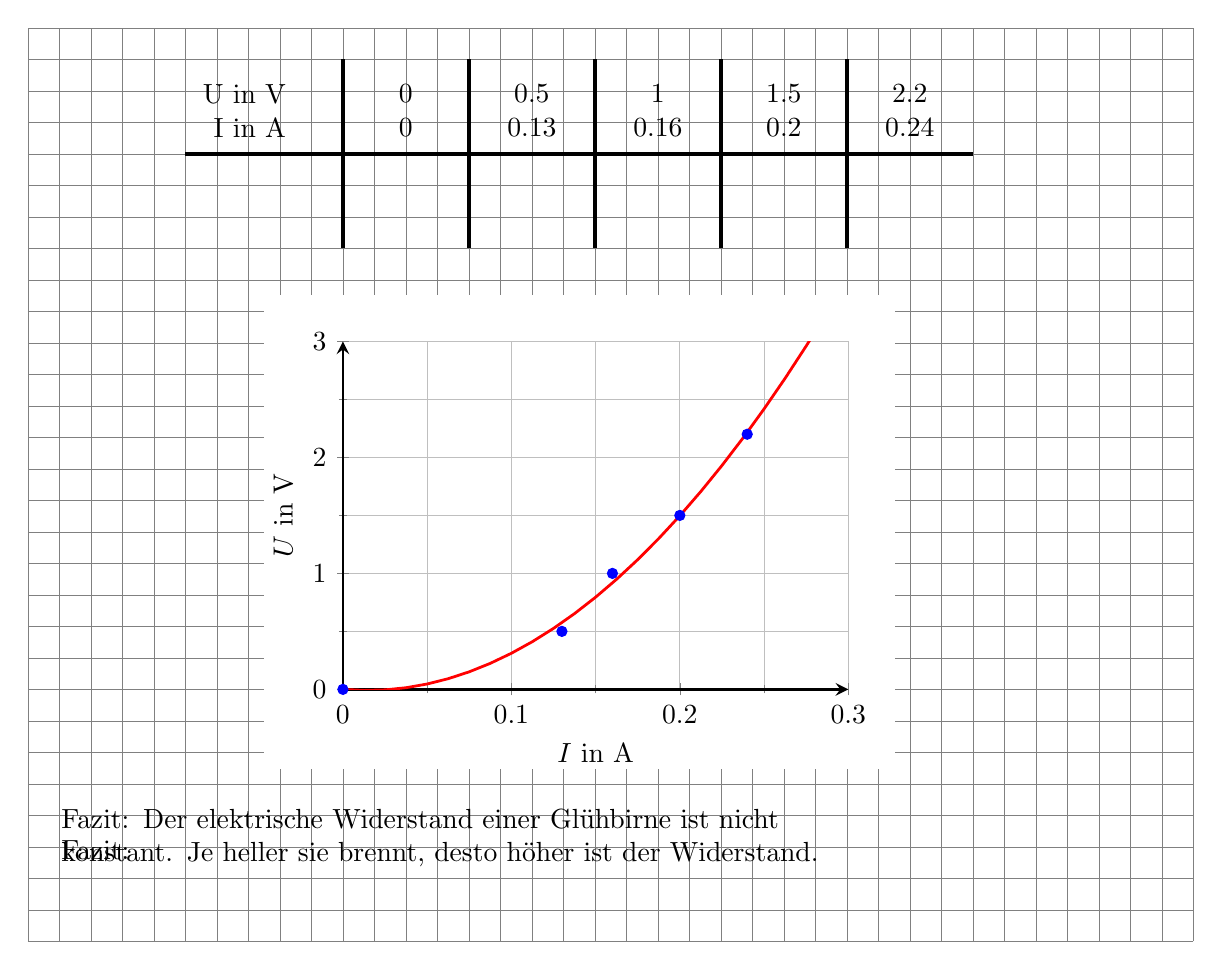
\begin{tikzpicture}
    \draw[step=4mm,gray,very thin] (0,0) grid (14.8,-11.6);


    \begin{scope}[shift={(1.2,0)}]
    \draw (2.2,-0.6) node[anchor=north east,align=right,text width=3cm] {%
  		\markertable%
        U in V
        \ \\
        I in A
        \ \\
    };

    \draw[very thick] (0.8,-1.6) -- ++(10,0);

    \draw[very thick] (2.8,-0.4) -- ++(0,-2.4);

    \draw (3.6,-0.6) node[anchor=north,align=center,text width=2cm] {%
  		\markertable%
        0
        \ \\
        \answer{0}
        \ \\
    };


    \draw[very thick] (4.4,-0.4) -- ++(0,-2.4);

    \draw (5.2,-0.6) node[anchor=north,align=center,text width=2cm] {%
  		\markertable%
        0.5
        \ \\
        \answer{0.13}
        \ \\
    };

    \draw[very thick] (6,-0.4) -- ++(0,-2.4);

    \draw (6.8,-0.6) node[anchor=north,align=center,text width=2cm] {%
  		\markertable%
        1
        \ \\
        \answer{0.16}
        \ \\
    };

    \draw[very thick] (7.6,-0.4) -- ++(0,-2.4);

    \draw (8.4,-0.6) node[anchor=north,align=center,text width=2cm] {%
  		\markertable%
        1.5
        \ \\
        \answer{0.2}
        \ \\
    };

    \draw[very thick] (9.2,-0.4) -- ++(0,-2.4);

    \draw (10,-0.6) node[anchor=north,align=center,text width=2cm] {%
  		\markertable%
        \answer{2.2}
        \ \\
        \answer{0.24}
        \ \\
    };
    \end{scope}

    \noanswer{
        \draw (0.3,-10.2) node[anchor=north west,align=left,text width=13cm] {%
      		\marker%
            Fazit:
        };
    }

    \answer{
        \draw (0.3,-9.8) node[anchor=north west,align=left,text width=13cm] {%
      		\marker%
            Fazit: Der elektrische Widerstand einer Glühbirne ist nicht\\
            konstant. Je heller sie brennt, desto höher ist der Widerstand.\\
        };
    }



    \begin{scope}[shift={(4,-8.4)}]
        \draw[color=white,fill=white] (-1,-1) rectangle (7,5);
        \begin{axis}[
                axis background/.style={fill=white},
                axis lines=left,
                xlabel=$I$ in A,
                ylabel=$U$ in V,
                xtick={0,0.1,0.2,0.3,0.4},
                ytick={0,1,2,3},
                minor tick num=1,
                grid=both,
                xmin=0.0, xmax=0.3,
                ymin=0, ymax=3,
                line width=1pt,
                height=6cm,
                width=8cm,
                domain=0:0.3,
            ]
            \answer{
                \addplot[
                    only marks,
                    mark=*,
                    mark size=1.5,
                    color=blue,
                ] coordinates
                {
                    (0,0)
                    (0.13, 0.5)
                    (0.16,1)
                    (0.2,1.5)
                    (0.24,2.2)
                };

                \addplot[
                    color=red,
                    domain=0:0.3,
                ] {43.736*x^2 - 1.2614*x};
            }
        \end{axis}
    \end{scope}

\end{tikzpicture}








\newpage
\experiment{Serieschaltung von Widerständen}

Baue das Experiment aus siehe \fref{fig:ohm_resistors_series} auf.

\begin{figure}[h!]
    \centering
    \includegraphics[width=6cm]{_images/ohm_widerstand_serie.pdf}
    \caption{Serieschaltung von Widerständen.}
    \label{fig:ohm_resistors_series}
\end{figure}

\begin{enumerate}
    \item Miss den Gesamtwiderstand der beiden Widerständen.
    \item Leite eine Formel für den Gesamtwiderstand her.
    \item Überprüfe deine Formel mit den anderen Widerständen.
\end{enumerate}

% Raster für die Antworten
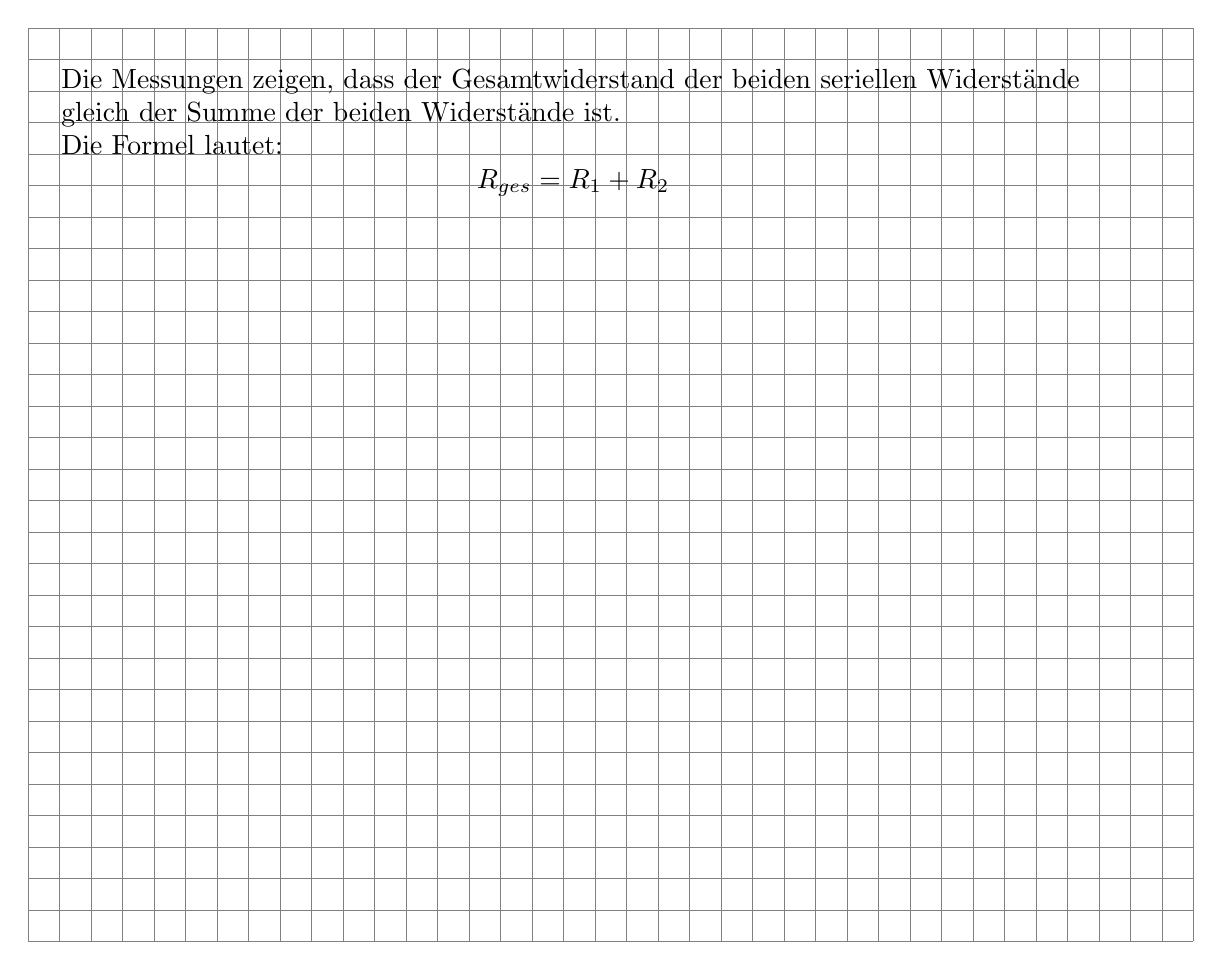
\begin{tikzpicture}
    \draw[step=4mm,gray,very thin] (0,0) grid (14.8,-11.6);

    \answer{
        \draw (0.3,-0.4) node[anchor=north west,align=left,text width=13cm] {%
      		\marker%
            Die Messungen zeigen, dass der Gesamtwiderstand der beiden
            seriellen Widerstände gleich der Summe der beiden Widerstände ist.

            Die Formel lautet:
            $$
            R_{ges} = R_1 + R_2
            $$
        };
    }

\end{tikzpicture}




\newpage
\experiment{Parallelschaltung von Widerständen}

Baue das Experiment aus siehe \fref{fig:ohm_resistors_parallel} auf.

\begin{figure}[h!]
    \centering
    \includegraphics[width=6cm]{_images/ohm_widerstand_parallel.pdf}
    \caption{Parallelschaltung von Widerständen.}
    \label{fig:ohm_resistors_parallel}
\end{figure}

\begin{enumerate}
    \item Miss den Gesamtwiderstand der beiden Widerständen.
    \item Leite eine Formel für den Gesamtwiderstand her.
    \item Überprüfe deine Formel mit den anderen Widerständen.
\end{enumerate}

% Raster für die Antworten
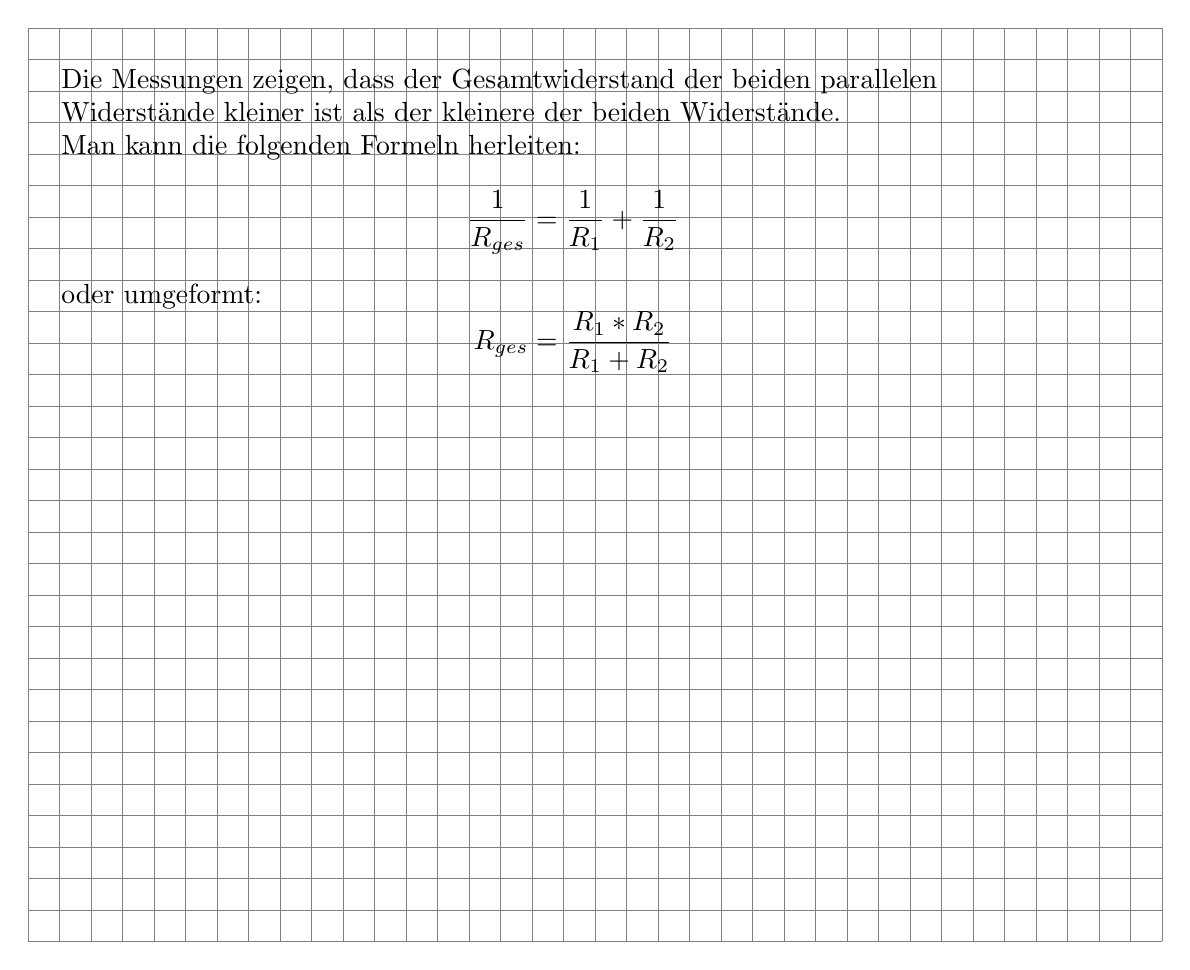
\begin{tikzpicture}
    \draw[step=4mm,gray,very thin] (0,0) grid (14.4,-11.6);

    \answer{
        \draw (0.3,-0.4) node[anchor=north west,align=left,text width=13cm] {%
      		\marker%
            Die Messungen zeigen, dass der Gesamtwiderstand der beiden
            parallelen Widerstände kleiner ist als der kleinere der beiden Widerstände.

            Man kann die folgenden Formeln herleiten:
            $$
            \frac{1}{R_{ges}} = \frac{1}{R_1} + \frac{1}{R_2}
            $$
            oder umgeformt:
            $$
            R_{ges} = \frac{R_1 * R_2}{R_1 + R_2}
            $$
        };
    }



\end{tikzpicture}
